\label{Konzept}
\chapter{Konzept}

Um sich auf die in \ref{Einleitung und Problemstellung} Einleitung und Problemstellung gennanten Zielgruppen (Personas \glqq Nutzer\grqq und \glqq Coach\grqq) einzulassen, hat man sich nach einiger Analyse entschieden, in einem ersten Schritt einen Chat-Bot zu programmieren, der basale Informationen vom Nutzer abfragt und den Bewerber einen Termin vereinbaren lässt. Weitere Iterationen sind nach erfolgreicher Beta-Phase möglich und ein Ausblick wird in \ref{Zusammenfassung und Ausblick} Zusammenfassung und Ausblick gegeben. Die Recherche ergibt ein Zweistufenmodell nach dem in einem ersten Schritt die Telegram Bot API genutzt wird, um einen Proof of Concept zu erstellen und eine geskriptete Variante des Bots zu schreiben, mit der der Approach getestet werden kann. In einem zweiten Schritt kann das BotMan Framework genutzt werden, um die Logik des Bots inkl. der bis dahin gesammelten Erfahrungswerte in eine Version 2 einfließen zu lassen, die mit weiteren Plattformen kompatibel ist und durch ihre bessere Skalierbarkeit auch kommerzialisiert werden könnte. Im Rahmen dieser Arbeit wird Schritt 1 des Zweistufenmodells umgesetzt.

\section{Grundkonzept, User Journey und Features} \label{Konzept: User Journey}
	Die Persona \glqq Nutzer\grqq  soll einen vordefinierten Workflow durchlaufen, der im Folgenden skizziert und im Abschnitt \ref*{Realisierung} näher beschrieben wird:

	\begin{enumerate}
		\item Ein Nutzer kommt entweder via Link oder durch die Telegram-Suchfunktion zum CoachingBot.\footnote{\url{https://t.me/thecoachingbot?start=start}}
		\item In Telegram angekommen öffnet sich ein neuer Chat mit dem CoachingBot.\footnote{Abhängig davon, ob der start-Zusatz schon in der URL inkludiert war oder nicht, muss jetzt der Befehl \/start eingegeben werden.}
		\item Der Bot stellt sich vor und beginnt eine Reihe an Fragen zu stellen. Antworten oder deren Format sind z.T. vordefiniert und werden vorgeschlagen.
		\item Der User teilt Texte, Bilder und andere Informationen.
        \item Sowohl Coach als auch Coachee sollen spätestens nach Abschluss des Konversationsflusses die Möglichkeit haben, eingegebene Daten einzusehen.
        \item Der Nutzer erhält seine Zusammenfassung automatisch nach der Stufe \verb|SUMMARY| via Chat sowie E-Mail und kann sie zusätzlich manuell vom Bot abfragen.
        \item Sobald alle Informationen eingereicht sind, erhält der Nutzer die Möglichkeit, einen Termin zu vereinbaren. Dem Nutzer werden dazu drei Terminvorschläge über die nächsten zehn Tage angeboten, aus denen er frei wählen kann. Die Dauer pro Termin beträgt 50 Minuten. Es können nur Termine ausgewählt werden, die noch nicht belegt sind und innerhalb der Geschäftszeiten liegen. (Auf die Auswahl der Zeitzone wird hier verzichtet, da das Coaching-Angebot aktuell nur in mitteleuropäischer Zeit angeboten wird.) Im Hintergrund wird ein Google Calendar gemanaged.
        \item Der Benutzer bekommt eine schriftliche Bestätigung in Form einer E-Mail mit dem vereinbarten Termin.\footnote{Sofern der Nutzer seinen Kalender so konfiguriert hat.} Darüber hinaus kann der Termin jederzeit vom Bot abgefragt werden.
        \item Der Bot verabschiedet sich. (Ende der Konversation)

    \end{enumerate}
	Der Prozess kann natürlich zu jeder Zeit unter- oder abgebrochen werden. Außerdem besteht die Möglichkeit für den Nutzer, seine Daten jederzeit einzusehen, zu löschen oder den Prozess neu zu starten.

	Für die Persona \glqq Coach\grqq  sollen eingereichte Informationen über alle Bewerber inkl. Termin in einer Übersicht im Web-Browser eingesehen werden können. Außerdem sind alle vereinbarten Termine auch im Calender des Coaches einsehbar.

\section{Technischer Aufbau}

	\begin{figure} %[hbtp]
		\centering
		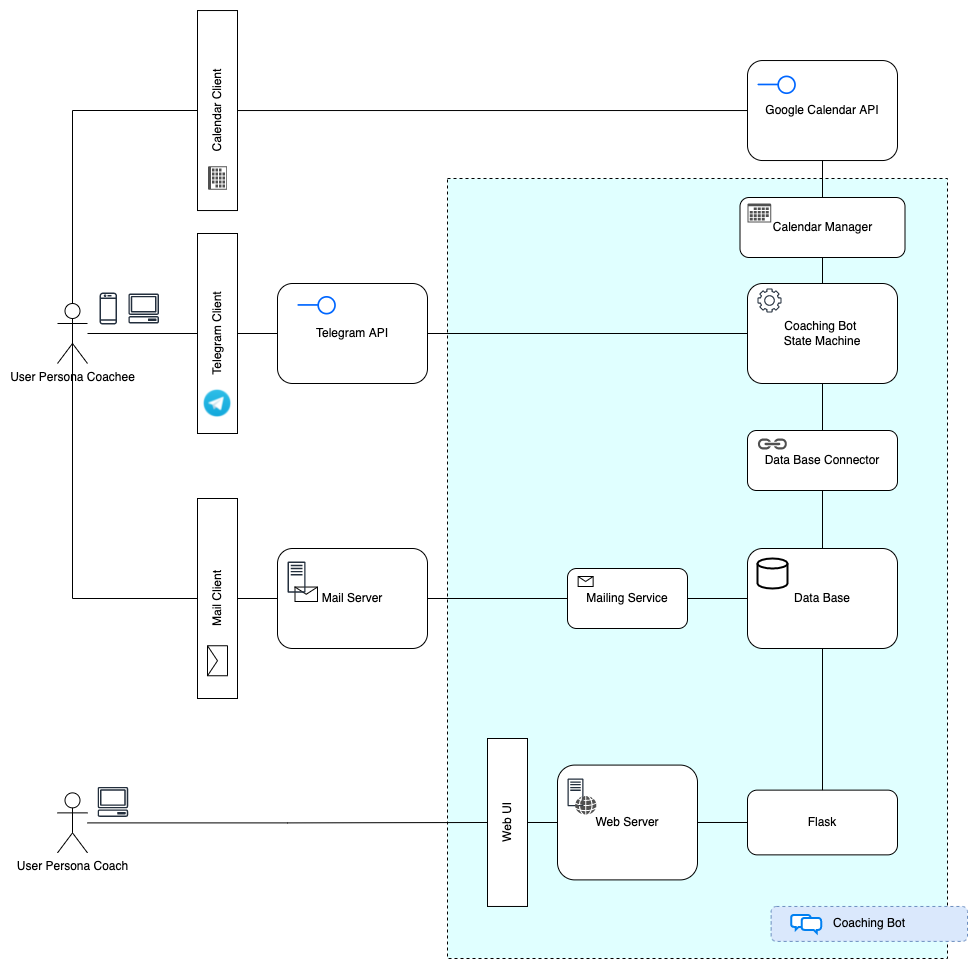
\includegraphics[width=1.0\textwidth]{images/220320_PA28464_Architecture.png}
		\caption{Konzeptionelle Architektur für das Projekt \emph{Der Coaching Bot}}
		\label{fig: architecture}
	\end{figure}

	Wie in Abbildung \ref{fig: architecture} rechts mittig skizziert, besteht der Kern des Bots aus einem endlichen Automaten (State Machine), der Zustände vordefiniert und festlegt, wann sich welcher Nutzer in welchem Zustand befindet und von welchem in welchen Zustand er sich wann bewegen darf. An diesen Kern sind als zentrales Steuerungselement des Bots alle anderen Systeme angebunden. Dazu gehören:
	\begin{enumerate}
		\item Die SQLite Datenbank zur Speicherung der Nutzerdaten
		\item Die Telegram API, über die die Kommunikation mit dem Telegram Client abgewickelt wird
		\item Die Google Calendar API, über die Events erstellt und versendet werden können
		\item Der Mail Server, über den E-Mails an den Nutzer versendet werden können.
	\end{enumerate} 

	Der Nutzer interagiert mit der Applikation durch drei Kanäle - in Abb. \ref{fig: architecture} links ersichtlich:
	\begin{enumerate}
		\item Telegram Client: Kommunikation mit dem Bot
		\item Calendar Client: Erhalt, Annahme sowie Ablehnung der vereinbarten Termine
		\item Mail Client: Erhalten der Zusammenfassung und Bestätigung
	\end{enumerate}
	
	Der Bot wird von Nutzern (in Abb. \ref{fig: architecture} links ersichtlich) via einem der verfügbaren Telegram Clients (Mobile oder Desktop) angesprochen und reagiert auf die Eingabe entsprechend. So können verschieden Funktionen ausgelöst werden. Bspw. werden Antworten zurückgegeben, Informationen gespeichert oder es wird ein Vorschlag gemacht und an den Nutzer zurückgegeben. Der Bot soll mit mehreren Benutzern gleichzeitig sprechen können. Das wird ermöglicht, weil alle Reaktionen des Bots mit der Kennung des jeweiligen Nutzers verknüpft sind. So spricht der Bot den Nutzer mit Namen an oder kann sich daran erinnern, welche Fragen schon beantwortet wurden und welche nicht. \\ \\
	
	Der Coach interagiert mit der Applikation nur durch einen Kanal (in Abb. \ref{fig: architecture} links unten ersichtlich) - den Web Browser. Hier steht eine einfache Übersicht über Anmeldungen, gesammelte Informationen und der aktuelle, monatliche Terminkalender zur Verfügung.\footnote{Der Kalender könnte auch über einen Calender-Client synchronisiert werden können.}

\section{Zustände \& Konversationsfluss}

	Im folgenden Zustandsdiagramm ist der Konversationsfluss des Bots auf hohem Abstraktionsniveau - als endlicher Automat (State Machine) - abgebildet. Es wird deutlich, dass der Bot einem Skript folgt und Loops soweit als möglich vermieden werden sollen. Der Haupt-Pfad ist fett eingezeichnet. Daneben besteht für die meisten Schritte die Möglichkeit für den Nutzer, eine Stufe zu überspringen, wenn er diese Angabe nicht machen möchte. Was aber, wenn der Nutzer den Vorgang unterbrechen möchte oder der Bot aufgrund eines technischen Grundes neu gestartet werden muss und der Nutzer erst danach wieder zur Konversation zurückkehrt? Es muss dem Nutzer möglich sein, dass nach einiger Zeit zum Bot zurückzukehren und an der Stelle weiterzumachen, an der er aufgehört hat. Zu diesem Zweck, dient der Zustand \verb|S0| (START) als zentraler Einstiegspunkt. Hier wird analysiert, ob der Nutzer schon bekannt ist und falls ja, bis wohin er den Prozess bereits durchlaufen hat. Dann wird er dorthin weitergeleitet. Daher ist es möglich von START aus zu allen anderen Zuständen zu gelangen, auch wenn das nicht die Regel ist. Hat der Nutzer den Prozess bereits abgeschlossen, so kann er sogar von S0 direkt in S10 (ENDE) landen und wird entsprechend benachrichtigt. Da dem Nutzer die Möglichkeit gegeben werden soll, den Prozess jederzeit zu beenden, ist es auch möglich, von jedem Zustand in \verb|S10| (ENDE) zu gelangen.\footnote{Der Konversationsfluss ist in einer sehr detaillierteren Ansicht verfügbar, in der der Unterschied zwischen dem hohen Abstraktionsniveau des Automaten und der Realität sichtbar wird. So lässt sich leicht erkennen, wo die Konversation beginnt und welche Zustände und Übergänge möglich sind: \url{https://github.com/mwel/coaching_bot/blob/main/thesis/images/220320_PA28464_Conversation_Flow.svg}} Übergänge sind nach dem im Abschnitt \ref{code: ConversationBot} ConversationBot skizzierten Format der \verb|state[n]|-Methoden aufgebaut. Eine detaillierte Beschreibung des Aufbaus dieser Methoden findet sich beispielhaft im Abschnitt \ref*{bio.py} Handler Funktionen. Der Nutzer löst die Übergänge durch seine Eingabe aus und wird dann durch die State Machine automatisch zum entsprechenden nächsten Zustand geleitet.
	Sobald der Bot gestartet wird, befindet er sich im Zustand S0.
	\begin{table} %[hbtp]
		\centering
		\begin{tabular}{l | l l l l}
			\textbf{Zustände} 	& \textbf{Beschreibung}\\
			\hline
			S0 					&		 START 			&		 Eingabe Biographie oder nächster Schritt oder Abbruch\\
			S1 					&		 BIO 			&		 Eingabe Geschlecht oder nächster Schritt oder Abbruch\\
			S2 					&		 GENDER 		&		 Eingabe Geburtsdatum oder nächster Schritt oder Abbruch\\
			S3 					&		 BIRTHDATE 		&		 Eingabe E-Mail Adresse oder Abbruch oder Abbruch\\
			S4 					&		 EMAIL 			&		 Eingabe Telefonnummer oder nächster Schritt oder Abbruch\\
			S5 					&		 TELEPHONE 		&		 Eingabe Ort oder nächster Schritt oder Abbruch\\
			S6 					&		 LOCATION 		&		 Eingabe Bild oder nächster Schritt oder Abbruch\\
			S7 					&		 PHOTO 			&		 Alle Daten angegeben oder übersprungen oder Abbruch\\
			S8 					&		 SUMMARY 		&		 Ausgabe Zusammenfassung\\
			S9 					&		 APPOINTMENT	&		 Terminvereinbarung oder Abbruch\\
			S10 				&		 ENDE 			&		 Ende: Applikation beendet (Neustart möglich)\\
			
		\end{tabular}
		\caption{Zustände des Konversationsflusses}
		\label{tab: states}
	\end{table}
	
	\begin{figure} %[hbtp]
		\centering
		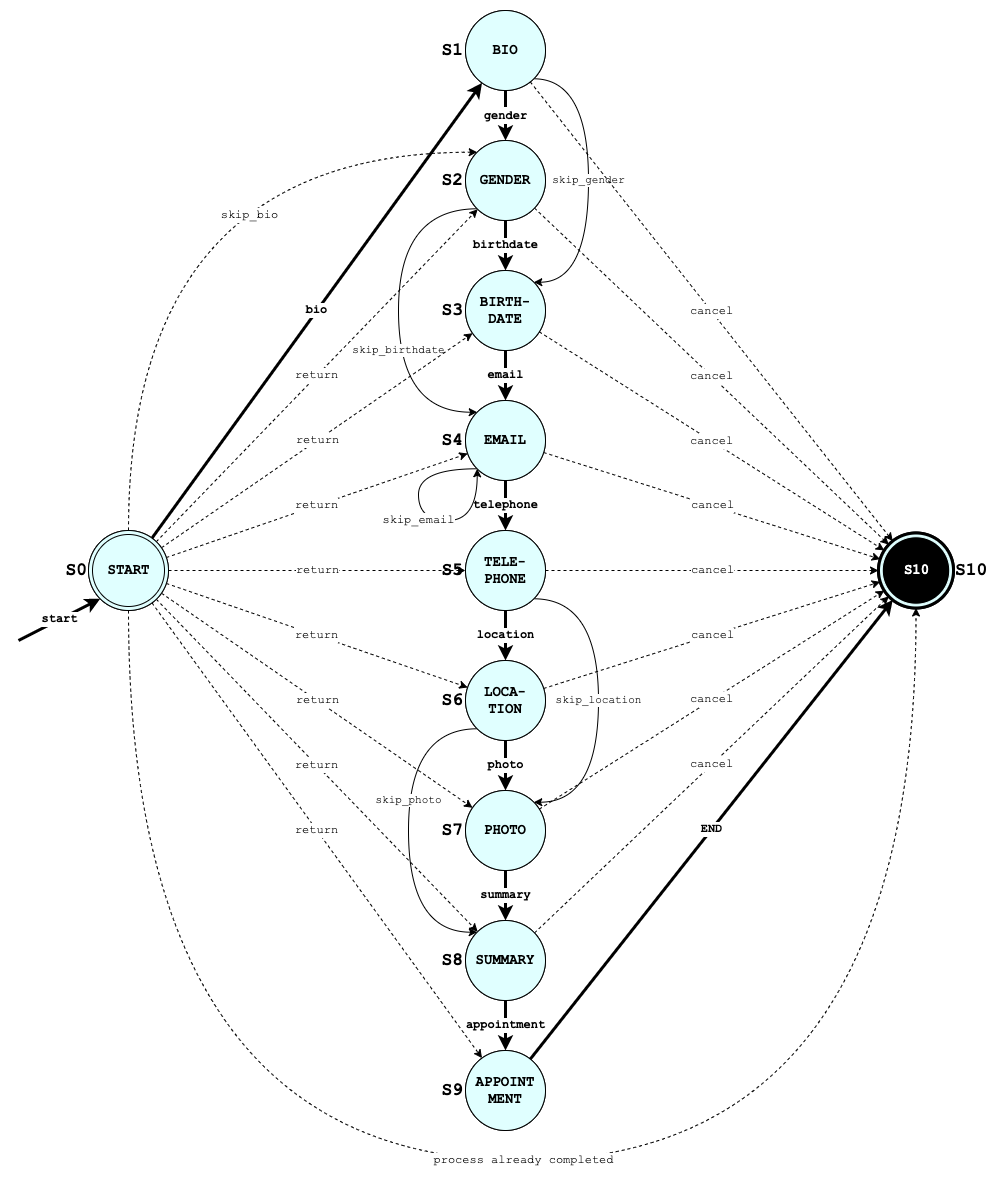
\includegraphics[width=1.0\textwidth]{images/220326_PA28464_State-Machine.png}
		\caption{Endlicher Automat des Konversationsflusses des Bots}
		\label{fig: state machine}
	\end{figure}
	